\part{Contextualização}

\chapter{Terapia Comunitária Integrativa}
A Terapia Comunitária Integrativa (TCI) surgiu em 1985 no bairro Pirambu, Fortaleza, CE, a partir de uma rede comunitária informal. Esse movimento nasceu da união de moradores, conectados por experiências compartilhadas, resultando na criação de uma prática terapêutica significativa. O fundador, Adalberto de Paula Barreto, doutor em psiquiatria, teologia e antropologia, desenvolveu a TCI com uma base interdisciplinar sólida, ancorada nos pilares do pensamento sistêmico, pragmática da comunicação humana, antropologia cultural, pedagogia de Paulo Freire e resiliência.\cite{BARRETO}

A metodologia da TCI é estruturada em fases como acolhimento, seleção da inquietação, contextualização, partilha de experiências e conclusão positiva. Criando um espaço protegido para a expressão e ressignificação das vivências individuais e coletivas. Resultados concretos evidenciam a transformação de carências em competências e a promoção da resiliência comunitária. \cite{SILVA}

A TCI vai além da promoção da saúde mental, manifestando como um catalisador para a construção de uma sociedade consciente, solidária e participativa. Sua abordagem inclusiva valoriza a diversidade cultural e as capacidades individuais, destacando-se como força motora na formação de sujeitos sociais ativos e conscientes de seu potencial transformador.\cite{BARRETO}

Além disso, a TCI responde à necessidade de uma abordagem psicossocial adaptável a diferentes contextos regionais. Nesses cenários, cada indivíduo reage a situações adaptando-se, seja alterando a própria abordagem, modificando o ambiente ao redor ou combinando essas duas operações em diferentes proporções.\cite{DANTAS} Destaca-se o papel de Adalberto no processo de expansão, desde apresentações em congressos até parcerias que propiciaram sua implantação em diversos países, colaborando com setores governamentais, não governamentais e privados.\cite{GOMES}

Praticada em mais de 24 países nas Américas, Europa e Ásia, a TCI é reconhecida pelo Ministério da Saúde como uma abordagem psicossocial avançada, vai além da esfera clínica, promovendo a construção de redes sociais solidárias, conexões e qualidade de vida. Inserida na Política Nacional de Práticas Integrativas e Complementares(PNPIC) desde 2017, a TCI integra conhecimento científico e sabedoria popular na busca de soluções para conflitos e sofrimentos humanos.\cite{ABRATECOM}

A Associação Brasileira de Terapia Comunitária Integrativa (ABRATECOM), autorizada por seu criador desde 2004, executa um papel fundamental nesse cenário. Atualmente, a ABRATECOM computa mais de 30.500 terapeutas comunitários em todo o Brasil, destacando a amplitude e o alcance dessa prática.\cite{SILVAFRANCO} Abaixo a distribuição geográfica dos Polos Formadores e de Cuidado credenciados pela\cite{ABRATECOM}:

\begin{figure}[!h] % ambiente usado para inserção de imagens
    \centering
    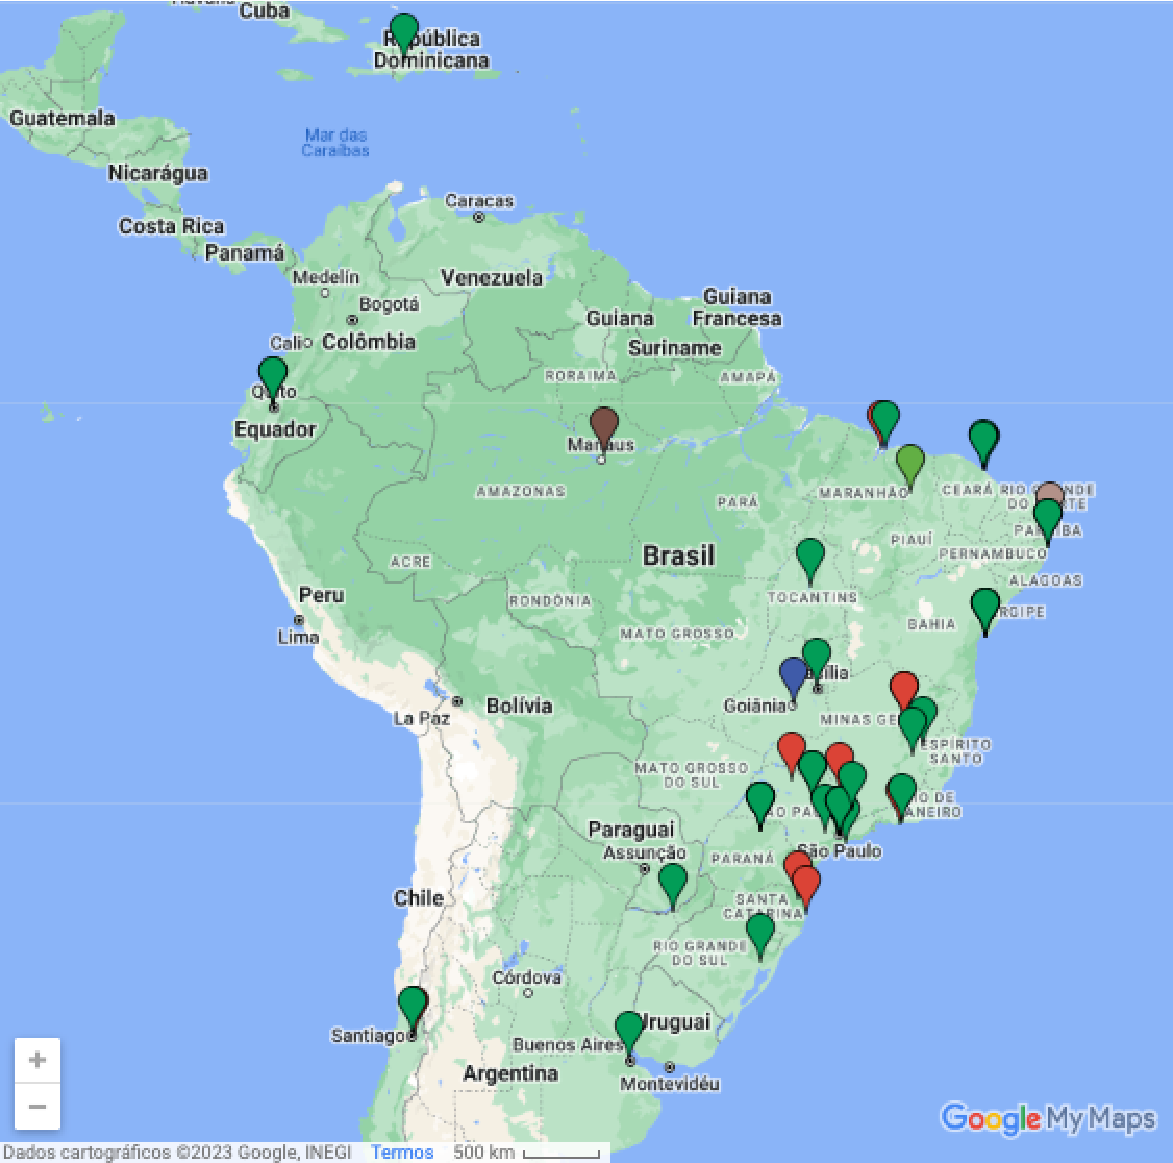
\includegraphics[scale=0.7]{latex/figuras/polos.pdf}
    \caption[Terapia Comunitária Integrativa]%seção
    {Distribuição de Polos Formadores e de Cuidado}%legenda
\end{figure}

A Terapia Comunitária Integrativa abraçou a era digital em 2020 diante dos desafios impostos pela pandemia da COVID-19. No Polo Formador Afinando Vidas, ocorreram rodas experimentais online para a criação e validação de um protocolo adaptado das etapas da TCI, que mais tarde foi replicado para os demais polos da ABRATECOM. Essa adaptação permitiu ressignificar a concepção de contato social e cuidado, promovendo uma nova e mais ampla forma de conexão sem alterar seus valores.\cite{SILVAeOTAVIANO}

Os valores que fundamentam a TCI são o acolhimento, a simplicidade, a circularidade do cuidado, a valorização das emoções, a ousadia e transgressão, a geração de dúvidas nas convicções, a horizontalidade das relações, a percepção do outro como recurso, a aceitação da imprevisibilidade e o amor com bom humor.\cite{SILVA}

Em um exemplo específico, durante 20 sessões de Terapia Comunitária Integrativa (TCI) realizadas entre agosto de 2018 e abril de 2019, \cite{BOARETTO} conduziram um estudo quase-experimental, sem distribuição aleatória, para avaliar os níveis de ansiedade e depressão em estudantes de graduação e pós-graduação. Utilizou-se a Escala de “Hospital Anxiety and Depression”, validada em português para o Brasil em 1995. Participaram 25 estudantes, divididos em quatro grupos (28\% pós-graduação, 72\% graduação), durante cinco sessões de TCI, com coleta de dados antes e depois das sessões. Todos eram adultos, com idades entre 19 e 29 anos, sendo a maioria do sexo feminino (84\%). Inicialmente, os escores para possível ansiedade eram de 52\%, e para depressão, de 12\%. Após as sessões de TCI, esses valores reduziram aproximadamente 53.85\% para ansiedade e 66.67\% para depressão.

\begin{figure}[!h] % ambiente usado para inserção de imagens
    \centering
    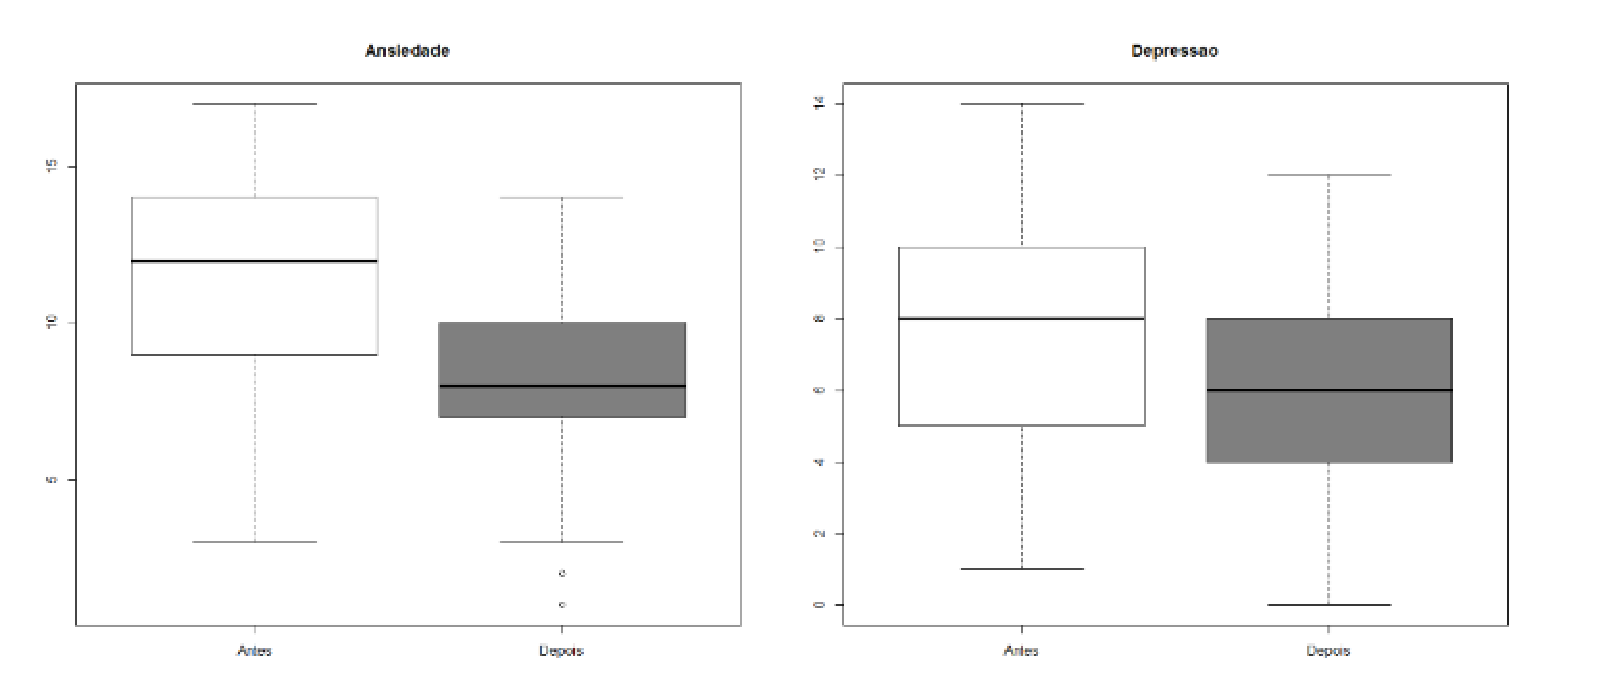
\includegraphics[scale=0.5]{latex/figuras/boaretto.pdf}
    \caption[Terapia Comunitária Integrativa]%seção
    {Comparação dos níveis do escore para ansiedade e depressão obtidos na pesquisa\cite{BOARETTO}}%legenda
\end{figure}

Ao analisar os dados, comparando os instrumentos aplicados antes e depois das cinco rodas de TCI, é possível verificar que mais da metade dos participantes apresentaram índices menores de ansiedade e depressão. Esse resultado tornou-se evidente ao término do estudo, quando os estudantes relataram uma redução da tensão, medo, inquietude e preocupação, juntamente com um aumento do ânimo, alegria e autoestima. Esses resultados destacam a necessidade e importância de programas de intervenção psicoterápica dentro das universidades.\cite{BOARETTO}

Em outra aplicação prática, indicadora dos benefícios da TCI, foi observada em uma pesquisa realizada para avaliar os efeitos antes e depois de uma única sessão. Um caso envolveu uma senhora que frequentava as rodas de forma assídua e enfrentava, em casa, de forma recorrente, a difícil situação de ter uma sobrinha envolvida com drogas, sendo essa sua única família. A sobrinha encorajada a participar da roda de TCI, permaneceu em silêncio durante toda a sessão, mas ao final, expressou que "a terapia não é um lugar de covardes". Sua avaliação antes da sessão refletia um estado emocional fragilizado, enquanto após a TCI, ela se sentia com disposição para explorar novas perspectivas e caminhos.\cite{LEITEePALOS} Essa experiência destaca a capacidade transformadora da TCI em situações complexas, proporcionando não apenas um espaço de expressão, mas também potencializando a perspectiva de mudança e crescimento. 



\chapter{Engenharia Eletrônica na Saúde Mental: Inovações Tecnológicas e Transformação Terapêutica}
A constante preocupação com a saúde da população e os avanços tecnológicos permitiram o desenvolvimento e integração de recursos que aprimoram a eficiência do cuidado. Destaca-se a atuação e os avanços proporcionados pela engenharia eletrônica no cuidado com a saúde mental, moldando uma abordagem de intervenção que se estende do ambiente clínico para a vida diária do indivíduo. Essa expansão visa potencializar a eficácia dos tratamentos terapêuticos.

A engenharia eletrônica desempenha um papel essencial no comprometimento com a expansão e manutenção da saúde mental. O desenvolvimento de tecnologias inovadoras oferece uma contribuição significativa por meio de sensores, algoritmos de processamento de sinais, softwares avançados, equipamentos eletrônicos e dispositivos vestíveis (Wearables). Essas ferramentas proporcionam intervenções personalizadas e direcionadas, facilitando a atuação de profissionais da saúde mental com abordagens mais precisas.

As abordagens se estendem de maneiras ativas, transformando a percepção do tratamento de distúrbios mentais. Ao integrar a tecnologia como complemento, estudos de caso e exemplos práticos destacam um potencial revolucionário na transformação do panorama geral da saúde mental.

Os recentes avanços em Inteligência Artificial (IA) e Processamento de Linguagem Natural (PNL) transformaram a análise de notas clínicas e insights do Registro Eletrônico de Saúde (EHR). Um estudo britânico aplicou PNL e IA no tratamento da depressão, identificando padrões de comportamento que demandam intervenção. Ao prever crises em pacientes de saúde mental, a pesquisa revelou a viabilidade técnica dessas abordagens, destacando oportunidades de integração em ferramentas de apoio à decisão clínica local. \cite{MSOSA}

No campo da neuroestimulação elétrica, estudos oferecem uma abordagem inovadora para tratar distúrbios mentais, modulando diretamente a sincronia oscilatória e a conectividade entre regiões cerebrais específicas. Essa técnica promissora representa um avanço significativo no tratamento, atuando no nível cerebral para alterar circuitos envolvidos em distúrbios neuropsiquiátricos.\cite{LO}

Outro exemplo prático envolve a proposta de um Assistente de Monitoramento de Emoções e Mentalidade (EMMA), um chatbot eficiente para saúde mental. Utilizando Deep Learning para analisar emoções por meio de texto, voz e expressão facial, alcançou impressionantes 85\% de precisão. A implementação de tecnologia blockchain assegura a segurança dos registros eletrônicos, permitindo o compartilhamento seguro com profissionais de saúde. Essa abordagem visa uma gestão eficaz de problemas de saúde mental de forma mais presente e com menor demanda de recursos.\cite{EMMA}

Esses exemplos reforçam a importância da engenharia eletrônica no desenvolvimento de terapias avançadas, por meio de inovações tecnológicas, proporcionando soluções eficazes e personalizadas para o bem-estar emocional. Na abordagem psicossocial avançada, destaca-se a Terapia Comunitária Integrativa, recentemente adaptada para a forma online. A engenharia eletrônica desempenha um papel crucial no desenvolvimento de uma plataforma online, segura e eficiente, capaz de facilitar os encontros terapêuticos de forma remota. Isso inclui a possibilidade de gerenciar sessões e integrar tecnologias de comunicação, como sistemas de videoconferência, proporcionando uma experiência fluida para terapeutas comunitários e participantes.

A preocupação com a segurança da informação é primordial para engenheiros eletrônicos. Por isso, na construção de uma plataforma online, incorpora-se um compromisso rigoroso com a transparência no tratamento de dados sensíveis dos usuários. Esse compromisso abrange o respeito à privacidade, a consideração cuidadosa da necessidade e segurança dos dados coletados, e a intenção contínua de estar em conformidade com a Lei Geral de Proteção de Dados\cite{LGPD}. Essa abordagem reforça a confiança dos usuários na plataforma, assegurando que suas informações sejam tratadas com o mais alto padrão de tecnologias de segurança e em conformidade com as leis vigentes.

Adicionalmente, para a engenharia eletrônica, é essencial implementar uma análise de dados de usabilidade para a identificação e resolução de problemas, além de orientar as tomadas de decisões informadas. Essas decisões têm como objetivo identificar, otimizar, melhorar e manter o desempenho dos sistemas, impulsionando a inovação contínua. Essa abordagem é fundamental para assegurar que a plataforma seja intuitiva e facilite a interação dos usuários, atendendo, assim, às necessidades específicas requeridas pela TCI online.

Por meio de suas inovações, a engenharia eletrônica desempenha um papel vital na criação de intervenções personalizadas voltadas para o bem-estar emocional. Essa sinergia entre tecnologia e a dedicação ao cuidado mental possibilita a elaboração de uma plataforma destinada ao gerenciamento das sessões online de Terapia Comunitária Integrativa. Nessa abordagem pioneira, a engenharia eletrônica não apenas estabelece uma base robusta, mas também facilita e aprimora a experiência de cada participante de maneira significativa.

